\documentclass[12pt]{article}

% Packages
\usepackage[utf8]{inputenc}
\usepackage{amsmath}
\usepackage{amsfonts}
\usepackage{amssymb}
\usepackage{graphicx}
\usepackage{hyperref}
\usepackage{tikz}
\usepackage{fancyvrb}
\usepackage{multicol}
\usepackage{array}
\usepackage{amsmath}
\usepackage{tabularx}
\usepackage{tcolorbox}

\usetikzlibrary{arrows.meta}
\hypersetup{
    colorlinks=true,
    linkcolor=black,
    citecolor=black,
}



% Document
\begin{document}

\title{Comparison in Concurrency Models in different programming languages}
\author{
    Christofer Washington Berruz Chungata \\ 
    Karan Jain \\ 
    Amey Makarand Dhongade \\ 
    \\
    San Jos\'{e} State University \\ 
    CS 252 - Final Project
}
\date{May 12, 2025}

\maketitle

\begin{abstract}
This project is very abstract
\end{abstract}

\section{Introduction\label{sec:introduction}}
This is my introduction

\section{Background\label{sec:background}}
Background.

\section{Shared-Memory Model\label{sec:shared_memory}}
A shared-memory concurrency model is any model in which units of computation,
processes or threads, communicate with each other using shared memory.
Communication is done by reading and writing to a shared object. Refer to
\autoref{fig:shared_memory} for a visual representation of the shared-memory model.

% shared memory figure
\begin{figure}[!htp]
    \centering
    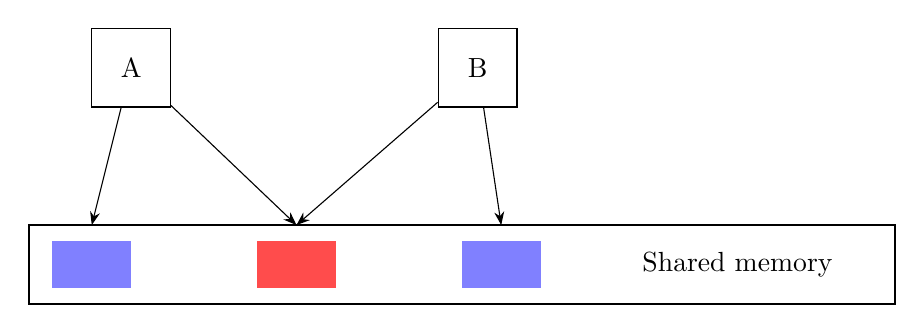
\begin{tikzpicture}[node distance=1cm and 1.5cm, >=Stealth]

        % Shared memory bar
        \draw[thick] (0,0) rectangle (11,1);
        \node at (9,0.5) {Shared memory};
      
        % Memory blocks
        \fill[blue!50] (0.3,0.2) rectangle (1.3,0.8);
        \fill[red!70] (2.9,0.2) rectangle (3.9,0.8);
        \fill[blue!50] (5.5,0.2) rectangle (6.5,0.8);
      
        % Processes A and B
        \node[draw, minimum width=1cm, minimum height=1cm] (A) at (1.3,3) {A};
        \node[draw, minimum width=1cm, minimum height=1cm] (B) at (5.7,3) {B};
      
        % Arrows from processes to memory blocks
        \draw[->] (A) -- (0.8,1);
        \draw[->] (A) -- (3.4,1);
        \draw[->] (B) -- (3.4,1);
        \draw[->] (B) -- (6.0,1);
      
      \end{tikzpicture}
      \caption{
        Shared-memory concurrency model. 
        Processes A and B communicate by reading and writing to shared memory blocks.
      }
      \label{fig:shared_memory}
\end{figure}

Note that the definition of \textit{memory} can be loosened depending on the application.
For example,~\cite{mitConcurrency} illustrates the following scenarios
where shared-memory concurrency models are applicable:

\begin{enumerate}
    \item A, B can be two processes communicating using the same process memory.
    \item A, B can be two programs communicating using the same filesystem.
    \item \label{itm:shared_object} A, B can be two running threads of some computer program
        communicating using the same object.
\end{enumerate}

When discussing limitations, advantages, or disadvantages of shared-memory concurrency models,
we will illustrate them using the scenario described in \autoref{itm:shared_object}.

\subsection{The Canonical Example}

The paper in~\cite{jaffe2011impactOfMemoryModels} describes a well-known canonical example.
Assume that we need to update a variable $x$ and increment it by $2$.
Assuming $x$ is already initialized, we can create two threads, $T_1$ and $T_2$, that will
increment $x$ by $1$ each. The code for both threads is shown in \autoref{fig:lost_update}.

Note that if both threads read the value of $x$ at the same time,
the final value of $x$ will be $1$. In fact, there's no guaranteed execution
order between $T_1$, and $T_2$ as the instructions can be interleaved
in any order. The interleaving problem is made more complex
due to the fact that most modern hardware can re-order instructions
\cite{huang2016debuggingConcurrentPrograms}. Furthermore, interleaving
makes it difficult to reproduce bugs, creating \textit{Heisenbugs}~\cite{rookout2021heisenbug,
gray1986whyComputersStop}.

\subsection{Problems with Shared-Memory Models}


%figure for the canonical example
\begin{figure}[!htp]
    \centering
    \begin{tabular}{|p{0.3\linewidth}|p{0.3\linewidth}|}
        \hline
        \textbf{$T_1$} & \textbf{$T_2$} \\
        \hline
        \begin{Verbatim}[fontsize=\small]
    int loc = x;
    loc = loc + 1;
    x = loc;
        \end{Verbatim}
        &
        \begin{Verbatim}[fontsize=\small]
    int loc = x;
    loc = loc + 1;
    x = loc;
        \end{Verbatim}
        \\
        \hline
    \end{tabular}
    \caption{Canonical example for shared-memory models.}
    \label{fig:lost_update}
\end{figure}


\section{Communicating Sequential Processes\label{sec:csp}}
CSP here
\section{Software Transaction Memory\label{sec:stm}}
STM here

% Bibliography
\bibliographystyle{plain}
\bibliography{references}

\end{document}